\section{Data}\label{sec:data}

\paragraph*{Stablecoin supply} Daily circulating supply comes from the DefiLlama stablecoins API~\cite{defillama}, with coin identifiers looked up by symbol. The primary aggregate $S_t$ sums \nCoins{} fiat-backed payment stablecoins (Table~\ref{tab:universe}): USDT, USDC, FDUSD, PYUSD, TUSD, USDP, BUSD (defunct, history retained), RLUSD, and three coins added under a rule fixed in the PAP (fiat-backed and above USD~1\,bn): USD1, USDG and USDGO. Tokenised money market funds (e.g.\ BUIDL) and crypto-collateralised or synthetic dollars (DAI/USDS, USDe) are excluded: the former are fund shares rather than payment stablecoins, and the latter are not backed by the cash-and-Treasury reserves that the Act regulates. Short gaps in a coin's series (up to three days) are forward-filled; across longer gaps the coin is excluded from the aggregate. The total of all USD-pegged coins reported by DefiLlama serves as a robustness aggregate.

\paragraph*{Timing} A DefiLlama snapshot dated $d$ is taken at 00:00~UTC and therefore measures supply at the end of US trading day $d-1$; we assign it accordingly. Assigning it to day $d$ is a pre-registered robustness check.

\paragraph*{Yields and controls} From FRED~\cite{fred} we take secondary-market Treasury-bill yields (4-week, 3-month, 6-month), constant-maturity 1- and 2-year yields, the effective federal funds rate, VIX, the S\&P~500 index and the Federal Reserve's overnight reverse repo (ON~RRP) volume. Yields are converted to basis points. The bitcoin closing price comes from Binance. All files are cached with download timestamps (vintage \vintage{}) and never edited by hand.

\paragraph*{Sample} The calendar is the set of US business days on which the 3-month bill yield is published. The estimation sample runs from \sampleStart{} to \sampleEnd{}: \nPre{} business days before enactment and \nPost{} after (\nPostTen{} at $h=10$). After alignment no regression variable has missing values. Fig.~\ref{fig:data} shows the series and Table~\ref{tab:stats} the summary statistics.

\begin{figure}[!t]
\centering
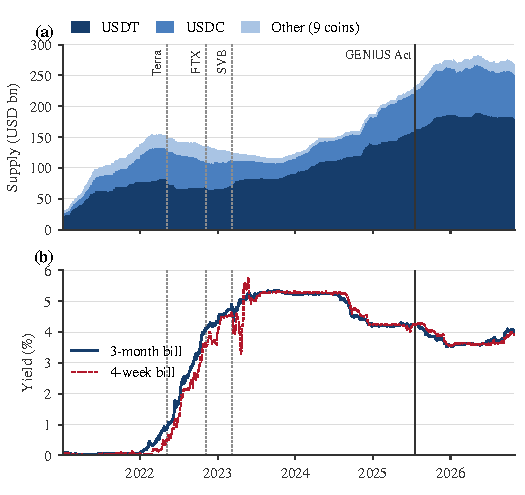
\includegraphics[width=\columnwidth]{figures/fig_data.pdf}
\caption{(a)~Circulating supply of the \nCoins{} fiat-backed USD stablecoins, by coin. (b)~Secondary-market yields on 4-week and 3-month Treasury bills. Daily, \sampleStart{} to \sampleEnd{}. Dotted lines: Terra depeg (9~May 2022), FTX collapse (8~Nov 2022), SVB closure (10~Mar 2023); solid line: GENIUS Act signed (18~Jul 2025). Sources: DefiLlama, FRED.}
\label{fig:data}
\end{figure}

The two regimes differ in ways that matter for interpretation. After enactment the average five-day inflow is smaller (USD~\flowMeanPost{}\,bn against \flowMeanPre{}\,bn) while its standard deviation is similar (\flowSDPost{} against \flowSDPre{}). Supply is about twice as large on average (USD~\supplyMeanPost{}\,bn against \supplyMeanPre{}\,bn). Daily changes in the 3-month yield are less volatile (standard deviation \dyThreeSDPost{}\,bp against \dyThreeSDPre{}\,bp). ON~RRP balances, a cushion of short-term liquidity before enactment (mean USD~\rrpPreMean{}\,bn), average only USD~\rrpPostMean{}\,bn afterwards.

\begin{table}[!t]
\centering
\caption{Summary statistics: mean (standard deviation)}
\label{tab:stats}
\footnotesize
\begin{adjustbox}{max width=\columnwidth}
% generated by src/viz/paper_tex.py
\begin{tabular}{lrr}
\toprule
 & Pre ($N=1135$) & Post ($N=322$) \\
\midrule
5-day flow $F_t$ (USD bn) & 0.90 (1.77) & 0.59 (1.91) \\
Supply $S_t$ (USD bn) & 135.47 (39.38) & 267.70 (11.98) \\
3-month bill yield (bp) & 316.80 (214.73) & 377.02 (19.58) \\
Daily $\Delta$ 3-month yield (bp) & 0.37 (3.73) & \ensuremath{-}0.07 (2.07) \\
2-year CMT yield (bp) & 316.13 (174.94) & 388.96 (40.64) \\
VIX & 19.58 (5.43) & 17.69 (3.12) \\
ON RRP (USD bn) & 1087.20 (819.77) & 14.09 (34.77) \\
\bottomrule
\end{tabular}

\end{adjustbox}
\end{table}
